% TODO: vymyslet lepší nadpisy

\section{Postup projektu}

V této sekci je popsáno praktické nasazení projektu \bso{}.

\subsection{Jedno-serverové nasazení}

První verze aplikace \bso{} využívala pouze jeden server pro hostování všech aplikačních funkcí jako \acrshort{webserver}, databázový server a aplikační server. Tento způsob hostování má však mnoho problémů.

Jelikož celá infrastruktura běží na jednom serveru narážíme na velké bezpečnostní riziko vytvářením kritického bodu infrastruktury, jehož nedostupnost nebo porucha znamená výpadek celé aplikace. 
To také znamená, že není možné aplikaci aktualizovat bez jejího výpadku. 

Druhým, i když menším problémem, je omezení možnosti škálování v~odpovědi na nárůst požadavků, jelikož pro alokaci větších serverových prostředků je nutné server vypnout.
Pro aplikaci \bso{} toto nepředstavovalo velký problém jelikož jazyk \acrshort{php} je velice efektivní ve využívání serverových prostředků a provoz aplikace nepřekročil alokované serverové prostředky.

\subsection{Více-serverové nasazení}

Pro vyřešení tohoto problému byla \hyperref[fig:servery]{infrastruktura byla rozšířena} na více serverů. 

Jako vstupní bod infrastruktury byl vyčleněn server označen \textit{gateway}.
Mezi hlavní role tohoto serveru byly určeny \hyperref[sub:load-balancing]{load-balancer} a vstupní bod protokolů \acrshort{http} a \acrshort{ws}.
To nám dovoluje provádět provizi ssl certifikátů a ssl terminaci pouze v jednom místě naší infrastruktury.

Jelikož \textit{gateway} poskytuje služby \hyperref[sub:load-balancing]{load-balanceru} mohlo být vytvořeno několik, na sobě nezávyslých, instancí aplikace \bso{}.
Pro provedení tohoto kroku bylo zapotřebí rozčlenit všechny zdroje dat, např. \acrshort{rdbms} nebo ukládání souborů, na dedikované servery, jelikož aplikační servery nemohou tyto služby mezi sebou sdílet.
Jako \acrshort{rdbms} byla využita spravovaná databáze společnosti Digitalocean s replikací a automatickou správou redundantních serverů.
Na ukládání souborů bylo využito objektové úložiště Amazon S3 pro manipulaci se soubory ze všech aplikačních serverů najednou, bez potřeby vlastní infrastruktury.

Rozčlenění aplikačních serverů nám poskytuje větší odolnost proti výpadku samostatných serverů, výpadek serveru neznamená výpadek aplikace, pouze zhoršení dostupnosti.
Také nám dovoluje aplikaci škálovat bez potřeby její odstávky.

\subsection{Problém s pracovními vlákny load-balanceru Nginx}

Při prvním veřejné výstavě uspořádané skrze platformu \bso{} docházelo při požadavcích na server k výpadkům a překročení časového limitu požadavku.
Po konzultaci souboru \verb|/var/log/nginx/access.log| bylo zjištěno, že na serveru \textit{gateway} došlo k vyčerpání \acrshort{fd}.
To vedlo k nemožnosti spracování požadavků serverem.

Pokud není webový server schopný odpovědět v časovém limitu zobrazí webový prohlížeč stránku jako nedostupnou,
jelikož webové prohlížeče implementují časový limit pro požadavky\cite{browser-timeout}.

Pro opravu této chyby bylo zapotřebí zvýšit počet požadavků spracovávaných jedním pracovním vláknem a horní limit \acrshort{fd}.
Tyto změny byly provedeny v souboru \verb|/etc/nginx/nginx.conf|.
Zvýšení počtu požadavků, které je schopné jedno pracovní vlákno spracovat bylo zvýšeno použitím direktivy.
\begin{verbatim}
events {
      worker_connections <počet připojení>;
}
\end{verbatim}
Pro zvýšení horního limitu \acrshort{fd} byla použita direktiva \verb|worker_rlimit_nofile <počet FD>|.

\section{Provoz a přínos aplikace}


Ve špičce provozu aplikace \bso{} využíval \hyperref[sub:load-balancing]{load-balancer} asi 30\si{Mb/S} síťového provozu.
Systém v~tu dobu navštívilo asi 790 návštěvníků, tj.\ kolem 25 návštěvníků na školu\footnote{Čísla nejsou exaktní z~důvodu nemožnosti přesného měření návštěvnosti webových stránek.}.

\subsection{Zapojení škol}

Během prvních 14-ti dní projektu se v Pardubickém Kraji, díky podpoře odboru školství, zapojilo více jak 60\% středních škol.
V ostatních krajích bylo, i přes podporu \acrshort{msmt}, zapojení škol pouze sporadické.
Pokrok ale nastal po zapojení Úřadu práce na celostátní úrovni, kdy jediný dopis informačním a poradenským střdiskům přinesl zapojení více než 250 škol z celé České Republiky.
Zapojení úřadu práce nám také poskytlo další komunikační kanál se základními školami.

\begin{figure}[h]
\centering
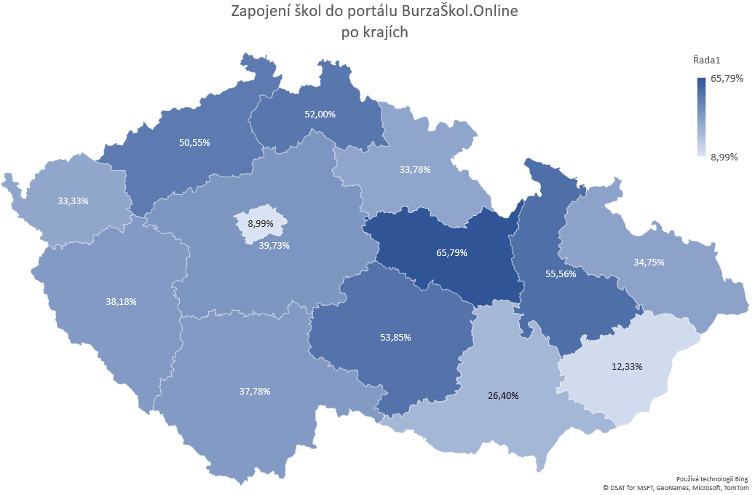
\includegraphics[width=\textwidth]{img/kraje-zapojeni.png}
\caption{Zapojení škol v jednotlivých krajích}
\label{fig:kraje-zapojeni}
\end{figure}

% tohle musí přesvědčit porotu o  tom, že si s nasazením nevymýšlíte.
% které bude na kolika serverech se to replikuje, jak vytížené jsou, jak vytížený je load-balancer,

\section{Přínos aplikace}

% tohle musí přesvědčit porotu o společenském přínosu, smysluplnosti aplikace 

% kolik v systému bylo škol, kdy byl nasazen poprvé a kolik se přes něj uskutečnilo spojení.
